%! Author = Omar Iskandarani
%! Date = 2/15/2025
\documentclass[a4paper,10pt]{article}
\usepackage{amsmath,amssymb,graphicx,hyperref,physics}
\usepackage[a4paper,margin=1in]{geometry}
\usepackage{array}
\usepackage{booktabs}
\geometry{margin=1in}


\title{The Vortex \AE ther Model: A Vorticity-Based Framework for Gravity and Electromagnetism}
\author{Omar Iskandarani}
\date{\today}

\begin{document}
    \maketitle

    \maketitle

    \begin{abstract}
        This paper introduces the Vortex \AE ther Model (VAM), a novel approach to fundamental physics where gravity and electromagnetism emerge from vorticity fields in an incompressible, inviscid \AE ther. The theory presented herein offers a modern interpretation of what is conventionally referred to as Æther theory, reimagined as a structured, inviscid superfluid medium governed by vorticity interactions rather than classical particulate motion. While the 19th-century concept of a luminiferous Æther was rejected following the Michelson-Morley experiment, the fundamental questions it sought to address—concerning the nature of space, energy propagation, and fundamental interactions—remain open. This work argues that a contemporary Ætheric model, grounded in fluid dynamics and topological vortex structures, may provide novel insights into quantum mechanics, inertia, and gravity.        Unlike General Relativity, which relies on spacetime curvature, VAM posits that gravitational attraction arises from pressure gradients induced by vortex filaments. Electromagnetism, in turn, is described as a consequence of structured vortex networks, with magnetic fields emerging from circulating Æther flows. Experimental predictions include measurable frequency shifts in rotating Bose-Einstein condensates and anomalous electromagnetic effects in high-vorticity plasmas. Proposed laboratory tests and detection methods are outlined to validate the Vortex Æther Model.        By extending Clausius’s thermodynamic principles into a vorticity-based gravitational model, this framework establishes a connection between classical thermodynamics, quantum mechanics, and fluid dynamics. Notably:        - Thermal expansion-contraction cycles of vortex knots mirror the behaviors observed in gas expansion laws.        - Energy transfer within the Æther follows structured vorticity dynamics, rather than being mediated by mass-energy interactions.        - Entropy-driven expansion aligns with cosmological models describing universal inflation without requiring dark energy.        This model offers a novel perspective on the nature of space, energy, and fundamental interactions, providing a coherent framework for future research into the unification of physical forces.
    \end{abstract}

    \section{Introduction}
    This model conceptualizes the vacuum as a non-viscous, dynamically evolving superfluid, fundamentally structured according to the five postulates of Euclidean geometry. The term Æther is employed here in its historical sense, as it has long been used to describe an all-pervading medium that facilitates energy transfer. However, in contrast to earlier mechanistic interpretations, this formulation eschews particulate motion in favor of continuous vorticity evolution. My conviction in this conceptualization was reinforced through an in-depth study of the original contributions of Maxwell \cite{maxwell1861}, Helmholtz \cite{helmholtz1858}, Kelvin \cite{kelvin1867}, and Clausius \cite{clausius1865}, whose works established the mathematical foundations for vortex dynamics and electromagnetic interactions.

    At the core of this model lies the concept of vortex knots—stable, topologically conserved rotational structures within the Æther. In particular, atomic structures are envisioned as self-sustaining vortex configurations, such as trefoil knots, encapsulated within spherical equilibrium boundaries. These knotted vortices exhibit a rigid-core structure, with surrounding potential flow regions exhibiting both rotational and irrotational components. The dynamics of these vortices are dictated by vorticity conservation principles, rather than mass-energy curvature. Experimental and theoretical advancements in vortex dynamics suggest that stable knotted vortices can persist in inviscid fluids \cite{kleckner2013}, reinforcing the notion that atomic structure may emerge from self-sustaining topological vortex configurations.

    Further experimental validation of this concept can be found in the behavior of superfluid helium, which exhibits quantized vortices that share striking similarities with the structured vorticity fields predicted by this model. Superfluid helium provides an example of an inviscid medium where vorticity exists in discrete, quantized states, reinforcing the plausibility of an Ætheric superfluid medium governed by similar principles \cite{vinen2002}. The interaction of these quantized vortices, as seen in superfluid turbulence, further supports the hypothesis that a vorticity-based framework can underpin fundamental physical interactions.

    A key departure from relativistic formulations is the assertion that time is absolute and flows uniformly throughout the Æther. However, local variations in vorticity influence time perception, as the rotational dynamics of vortex cores alter local energy distributions and equilibrium states. This provides an alternative to relativistic time dilation, where accelerations and vorticity gradients—not spacetime curvature—determine time flow differences. This approach finds further support in studies of vorticity in gravitomagnetism \cite{cahill2005}, where frame-dragging and precession effects emerge from rotating mass flows rather than from spacetime curvature. Thus, local time evolution is inherently tied to vorticity gradients and not relativistic spacetime warping.

    A central feature of this framework is the thermal expansion and contraction of vortex knots, a principle inspired by Clausius’s mechanical theory of heat. In this model, atoms and fundamental particles are represented as self-sustaining vortex configurations that exist within spherical equilibrium pressure boundaries. These knotted vortices interact dynamically with the surrounding Æther, expanding and contracting in response to thermal input, a process mathematically analogous to the expansion of gases under heat. This fundamental behavior links thermodynamics directly to vorticity, establishing entropy as a function of structured rotational energy. Studies on equilibrium energy and entropy of vortex filaments \cite{belik2023} provide strong evidence that vortical structures self-organize by redistributing kinetic energy through vorticity-driven entropy gradients, lending credibility to this perspective.

    Additionally, this model provides a natural bridge between quantum mechanics and vortex theory. The quantization of circulation in superfluid helium offers a direct analogy to the quantized nature of angular momentum in quantum mechanics, suggesting that elementary particles may arise from structured vortex dynamics in the Æther. The Schrödinger equation, often interpreted as governing probability waves, can instead be viewed as describing the stable, standing wave solutions of vortex structures in the Æther. This aligns with the observed wave-particle duality, where particles exhibit both localized (vortex core) and delocalized (potential flow) characteristics, depending on observational context. Furthermore, the emergence of discrete energy levels in atomic systems could be explained through resonant vortex interactions, where stable configurations correspond to eigenmodes of the vortex-boundary system.

    At the core of this model is the interaction between entropy, pressure equilibrium, and vortex stability. The spherical equilibrium boundary surrounding a vortex knot is hypothesized to behave elastically, responding to changes in rotational energy via:
    \begin{itemize}
        \item Thermal input → Expansion of the vortex boundary, reducing internal pressure and increasing the system’s entropy.
        \item Energy dissipation → Contraction of the vortex boundary, increasing core density and stabilizing vorticity distributions.
    \end{itemize}


    This process provides a thermodynamic foundation for vortex structure evolution, supporting a direct analogy between entropy variations and vortex interactions. The entropy of a vortex configuration is defined as:
    \begin{equation} \label{eq:Entropy}
        S \propto \int \omega^2 dV
    \end{equation}


    where:

    \begin{itemize}
        \item \( S \) is the entropy of the vortex configuration.
        \item \( \omega \)  is the local vorticity field.
        \item The integral is taken over the vortex volume.
    \end{itemize}

    This equation suggests that entropy is directly related to the vorticity distribution within the Æther, reinforcing the idea that vortex evolution follows thermodynamic principles, rather than requiring mass-energy curvature as in General Relativity.

    By extending Clausius’s thermodynamic principles into a vorticity-based gravitational model, this framework establishes a connection between classical thermodynamics, quantum mechanics, and fluid dynamics. Notably:

    \begin{itemize}
        \item Thermal expansion-contraction cycles of vortex knots mirror the behaviors observed in gas expansion laws.
        \item Energy transfer within the Æther follows structured vorticity dynamics, rather than being mediated by mass-energy interactions.
        \item Entropy-driven expansion aligns with cosmological models describing universal inflation without requiring dark energy.
    \end{itemize}

    Part I of this work will present foundational considerations, articulated with the intention of minimizing the necessity for advanced mathematical understanding, thereby making the content accessible to a broader audience. Part II will delve into the mathematical formalism underpinning the model, utilizing approaches such as the Bragg-Hawthorne equation in spherical symmetry \cite{keller2024} to formalize the equilibrium dynamics of vortex-driven Æther structures. The ultimate objective is to establish the foundations for a comprehensive non-viscous liquid Æther theory, capable of providing a visual and conceptual representation of inertia as an emergent property of vortex circulation within the Æther, particularly influenced by the proposed constants and the conservation of helicity \cite{kleckner2016}.





    This model offers a novel perspective on the nature of space, energy, and fundamental interactions, providing a coherent framework for future research into the unification of physical forces.

        \begin{table}[h]
            \centering
            \renewcommand{\arraystretch}{1.3}
            \begin{tabular}{c l}
                \toprule
                Symbol & Description \\
                \midrule
                \( V \) & Mass of liquid in circular motion (Vortex) \\
                \( \Gamma \) & Circulation: \( \oint \mathbf{v} \cdot d\mathbf{s} \) \\
                \( \omega \) & Vorticity magnitude \(\nabla \times \mathbf{v} \) \\
                \( \Phi \) & Vorticity-induced potential function \\
                \( R \) & Characteristic vortex radius \\
                \( L \) & Rotational vortex core length \\
                \( \Psi \) & Stream function of vortex motion \\
                \( \rho \) & Fluid density \\
                \( \mathbf{v} \) & Velocity vector field \\
                \( \mathbf{\Omega} \) & Angular velocity vector \\
                \( H \) & Helicity: \( \int \mathbf{v} \cdot \mathbf{\omega} \, dV \) \\
                \( K \) & Enstrophy: \( \int \omega^2 \, dV \) \\
                \bottomrule
            \end{tabular}
            \caption{Glossary of Terms for Incompressible Non-Viscous Liquid Æther}
            \label{tab:notation}
        \end{table}



        \begin{table}[h]
            \centering
            \renewcommand{\arraystretch}{1.3}
            \begin{tabular}{c l}
                \hline
                Symbol & Description \\
                \hline
                \( \Gamma \) & Vortex circulation strength, defined as \( \Gamma = \oint_C \mathbf{v} \cdot d\mathbf{s} \). \\                \( \omega \) & Vorticity magnitude, given by \( \omega = \nabla \times \mathbf{v} \). \\
                \( R \) & Characteristic vortex radius, representing the scale of rotation. \\
                \( \Phi \) & Vorticity-induced potential function, satisfying \( \nabla^2 \Phi = -\omega \). \\
                \( \Psi \) & Stream function for incompressible flow, where \( \mathbf{v} = \nabla \times \Psi \). \\
                \( H \) & Helicity, a measure of the knottedness of vortex tubes: \( H = \int \mathbf{v} \cdot \mathbf{\omega} \, dV \). \\
                \( K \) & Enstrophy, representing rotational energy density: \( K = \frac{1}{2} \int \omega^2 dV \). \\
                \( \rho \) & Local Æther density, assumed to be incompressible in the model. \\
                \( p \) & Pressure in the Æther model, often governed by Bernoulli-like principles. \\
                \( \mathbf{A} \) & Vector potential, where \( \mathbf{B} = \nabla \times \mathbf{A} \) in magnetohydrodynamic analogies. \\
                \( \mathbf{J} \) & Vortex current density, defined by \( \mathbf{J} = \nabla \times \omega \). \\
                \( \lambda \) & Vortex core parameter, related to the characteristic decay length of vorticity. \\
                \( \Psi_k \) & Vortex knot function describing topological structures in the Æther. \\
                \hline
            \end{tabular}
            \caption{Notation for the incompressible non-viscous Æther model.}
            \label{tab:notation2}
        \end{table}


    \section{Part I: 1. The demand for an extension for the propositions of physics}\label{sec:introduction}

A comprehensive examination of physical theory necessitates a clear distinction between objective reality, which exists independently of theoretical constructs, and the physicist's formulations that aim to describe it. These formulations, as approximations, endeavor to construct an intelligible representation of the universe. By identifying patterns in nature and employing mathematical and philosophical frameworks to predict outcomes, physics has developed diverse branches that, while initially disparate, have revealed profound interconnections.

Contemporary scientific paradigms are dominated by the Theory of Relativity and Modern Physics, which describe reality under narrowly defined conditions—notably the behavior of clocks and measuring rods, and the statistical properties of electrons. However, these frameworks neglect the æther, explicitly excluding it in favor of relativistic interpretations. The present model proposes a non-relativistic, vorticity-centric approach, highlighting the insufficiency of Relativity and Modern Physics in capturing the æther’s objective reality. While Relativity excels in describing phenomena like clock rotation, its applicability is confined to a limited domain.

Relativity defines simultaneity through synchronized clocks and exchanged light signals. This concept requires revision in a non-relativistic æther framework, particularly as quantum entanglement suggests non-local mechanical information transfer beyond the speed of light. Thus, simultaneity in the æther must account for these phenomena, enabling a more comprehensive understanding of temporal relationships.

The non-viscous liquid æther model posits that variations in atomic temporal experiences, reflected in clock synchronization discrepancies, arise from the vorticity and internal dynamics of vortex knots. These structures govern temporal differentiation through conserved constants. For instance, the hydrogen atom’s nucleus—the proton—is modeled as a spherical pressure equilibrium enclosing a trefoil knot vortex. This simplest and most stable configuration exemplifies atomic nuclei. The tangential velocity at the vortex boundary is constrained by angular velocity constants, with the speed of light as an upper limit for æther particle velocities.

Knot theory provides a critical mathematical framework for analyzing vortex knots in fluid systems, including the æther. Research has established that helicity—a conserved quantity in ideal fluid dynamics—is analogous to quantum spin, linking macroscopic fluid phenomena with atomic-scale behavior. Stable knotted structures, such as trefoil knots, exhibit robust energy distribution and stability, underscoring their fundamental role in matter’s architecture.

These knotted configurations in the æther are inherently dynamic, facilitating energy and angular momentum exchange with their surroundings. Their behavior adheres to the Navier-Stokes equations for inviscid, incompressible flows, modified by absolute vorticity conservation constraints. This dynamism enables the model to address complex interactions within the æther framework.

Future investigations will incorporate topological invariants, such as linking numbers and higher-order polynomial measures, to quantify vortex knottedness. These invariants correlate directly with measurable quantities like energy, momentum, and angular momentum, providing a bridge between theoretical constructs and empirical observations. By establishing these connections, the model could yield novel insights into quantum field interactions and macroscopic phenomena, potentially unifying disparate domains of physics.

Expanding the scope of physical propositions to encompass dynamical systems, helicity dynamics, and nonlinear æther interactions offers a pathway to reconcile fluid dynamics with quantum mechanics. This approach maintains a foundation in Euclidean spatial geometry and absolute time, advancing a cohesive framework that transcends the limitations of existing relativistic and quantum paradigms.




    \section{Mathematical Formulation of VAM}\label{sec:mathematical-formulation-of-vam}

    \subsection{Vorticity Transport Equation}\label{subsec:vorticity-transport-equation}
    \begin{equation} \label{eq:vorticity}
        \frac{D\boldsymbol{\omega}}{Dt} = (\boldsymbol{\omega} \cdot \nabla) \mathbf{v} - \boldsymbol{\omega} (\nabla \cdot \mathbf{v})
    \end{equation}


    \subsection{Biot-Savart Law for Vortex Filaments}\label{subsec:biot-savart-law-for-vortex-filaments}
    \begin{equation}
        \mathbf{v}(\mathbf{r}) = \frac{1}{4\pi} \int \frac{\boldsymbol{\omega} \times (\mathbf{r} - \mathbf{r'})}{|\mathbf{r} - \mathbf{r'}|^3} d^3\mathbf{r'}\label{eq:equation}
    \end{equation}

    \subsection{Bernoulli Equation and Gravity}\label{subsec:bernoulli-equation-and-gravity}
    \begin{equation}
        P + \frac{1}{2} \rho v^2 + \rho \Phi = \text{constant}\label{eq:equation2}
    \end{equation}

    \subsection{Photon Frequency as a Function of Vortex Circulation}\label{subsec:photon-frequency-as-a-function-of-vortex-circulation}
    \begin{equation}
        f = \frac{\Gamma}{2\pi R}\label{eq:equation3}
    \end{equation}


    \begin{figure}[h]
        \centering
        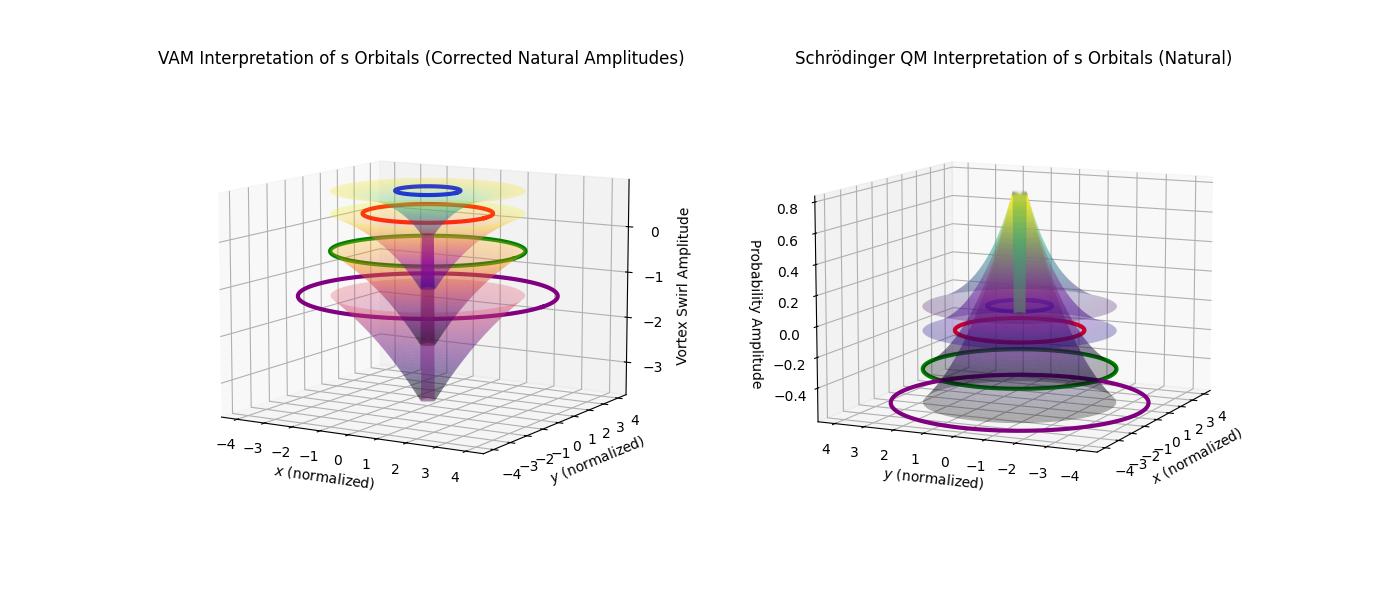
\includegraphics[width=0.7\textwidth]{vortex_diagram}
        \caption{Illustration of a vortex filament in Æther.}
        \label{fig:vortex}
    \end{figure}


    \section{Gravity as a Vorticity-Induced Pressure Gradient}\label{sec:gravity-as-a-vorticity-induced-pressure-gradient}
    - Gravitational attraction follows naturally from vortex pressure fields.
    - No singularities; replaces the concept of mass curvature with rotational fluid dynamics.

    \section{Electromagnetism as a Vortex Filament Network}\label{sec:electromagnetism-as-a-vortex-filament-network}
    - Reformulation of Maxwell’s Equations in terms of vorticity.
    - Magnetic field as a direct consequence of circulating \AE ther flows.

    \section{Experimental Predictions and Feasibility}\label{sec:experimental-predictions-and-feasibility}
    - Using rotating Bose-Einstein condensates (BECs), we predict vortex filaments to exhibit a circulation-dependent frequency shift measurable via phase-contrast imaging~\cite{kleckner2013}.

    - Electromagnetic anomalies predicted for high-vorticity plasmas.
    - Proposed laboratory tests and detection methods~\cite{kleckner2013, vinen2024, podkletnov2007, orlandi2021}.

    \section{Conclusion}\label{sec:conclusion}
    We have outlined a vortex-based approach to gravity and electromagnetism, As shown in Eq. \eqref{eq:vorticity}, the vorticity transport equation governs  The Vortex \AE ther Model offers a new perspective on fundamental forces,
    replacing spacetime curvature with fluid dynamics in an inviscid \AE ther.
    This framework provides a coherent mathematical model with experimentally testable predictions.
    While VAM provides an alternative to spacetime curvature, further work is needed to derive cosmological implications.
    How does VAM handle large-scale structure formation?
    Can it explain galactic rotation curves without dark matter?
    Future research will explore these avenues.

% Table of Physical Constants used in the Vortex Æther Model
    \begin{table}[h]
        \centering
        \renewcommand{\arraystretch}{1.2}
        \begin{tabular}{lllc}
            \toprule
            \textbf{Symbol} & \textbf{Value} & \textbf{Unit} & \textbf{Quantity} \\
            \midrule
            $C_e$ & $1.09384563 \times 10^6$ & $\text{m s}^{-1}$ & Vortex-Core Tangential Velocity \\
            $F_{\text{max}}$ & $29.053507$ & $\text{N}$ & Maximum Force \\
            $F_c$ & $29.053507$ & $\text{N}$ & Centrifugal Force \\
            $R_c$ & $1.40897017 \times 10^{-15}$ & $\text{m}$ & Coulomb Barrier \\
            $r_c$ & $1.40897017 \times 10^{-15}$ & $\text{m}$ & Vortex-Core Radius \\
            $R_e$ & $2.8179403262 \times 10^{-15}$ & $\text{m}$ & Classical Electron Radius \\
            $c$ & $2.99792458 \times 10^8$ & $\text{m s}^{-1}$ & Speed of Light in Vacuum \\
            $\alpha_g$ & $1.7518 \times 10^{-45}$ & - & Gravitational Coupling Constant \\
            $\mu_0$ & $4\pi \times 10^{-7}$ & $\text{N A}^{-2}$ & Vacuum Magnetic Permeability \\
            $\varepsilon_0$ & $8.854187817 \times 10^{-12}$ & $\text{F m}^{-1}$ & Vacuum Electric Permittivity \\
            $Z_0$ & $376.730313412$ & $\Omega$ & Characteristic Impedance of Vacuum \\
            $G$ & $6.67430 \times 10^{-11}$ & $\text{m}^3 \text{kg}^{-1} \text{s}^{-2}$ & Newtonian Constant of Gravitation \\
            $h$ & $6.62607015 \times 10^{-34}$ & $\text{J Hz}^{-1}$ & Planck Constant \\
            $\hbar$ & $1.054571817 \times 10^{-34}$ & $\text{J s}$ & Reduced Planck Constant \\
            $L_p$ & $1.616255 \times 10^{-35}$ & $\text{m}$ & Planck Length \\
            $M_p$ & $2.176434 \times 10^{-8}$ & $\text{kg}$ & Planck Mass \\
            $t_p$ & $5.391247 \times 10^{-44}$ & $\text{s}$ & Planck Time \\
            $T_p$ & $1.416784 \times 10^{32}$ & $\text{K}$ & Planck Temperature \\
            $e$ & $1.602176634 \times 10^{-19}$ & $\text{C}$ & Elementary Charge \\
            $\alpha$ & $7.2973525643 \times 10^{-3}$ & - & Fine-Structure Constant \\
            $R_\infty$ & $1.0973731568157 \times 10^7$ & $\text{m}^{-1}$ & Rydberg Constant \\
            $A_0$ & $5.29177210903 \times 10^{-11}$ & $\text{m}$ & Bohr Radius \\
            $M_e$ & $9.1093837015 \times 10^{-31}$ & $\text{kg}$ & Electron Mass \\
            $M_{\text{proton}}$ & $1.67262192369 \times 10^{-27}$ & $\text{kg}$ & Proton Mass \\
            $M_{\text{neutron}}$ & $1.67492749804 \times 10^{-27}$ & $\text{kg}$ & Neutron Mass \\
            $k_B$ & $1.380649 \times 10^{-23}$ & $\text{J K}^{-1}$ & Boltzmann Constant \\
            $R$ & $8.314462618$ & $\text{J mol}^{-1} \text{K}^{-1}$ & Gas Constant \\
            $\lambda_c$ & $2.42631023867 \times 10^{-12}$ & $\text{m}$ & Electron Compton Wavelength \\
            $\Phi_0$ & $2.067833848 \times 10^{-15}$ & $\text{Wb}$ & Magnetic Flux Quantum \\
            $eV$ & $1.602176634 \times 10^{-19}$ & $\text{J}$ & Electron Volt \\
            \bottomrule
        \end{tabular}
        \caption{List of Physical Constants Used in the Vortex \AE ther Model (VAM)}
        \label{tab:vam_constants}
    \end{table}


    \section{Validated VAM Equations}\label{sec:validated-vam-equations}
    \begin{align}$$
                \begin{equation}
                R_e &= \frac{\lambda_c}{2 \pi} \alpha \\\label{eq:equation4}
                \end{equation}
                \begin{equation}
                R_e &= \frac{e^2}{4 \pi \varepsilon_0 M_e c^2} \\\label{eq:equation5}
                \end{equation}
                \begin{equation}
                R_e &= 2 r_c \\\label{eq:equation6}
                \end{equation}
                \begin{equation}
                R_e &=  \alpha^2 a_0 \\\label{eq:equation7}
                \end{equation}
                \begin{equation}
                R_e &= \frac{e^2}{4 \pi \varepsilon_c m_c c^2} \\\label{eq:equation9}
                \end{equation}
                \begin{equation}
                R_e &= \frac{e^2}{8 \pi \varepsilon_0 F_{\text{max}} r_c} \\\label{eq:equation8}
                \end{equation}
                \begin{equation}
                R_x &= N \frac{F_{\max} r_c^2}{M_e Z C_e^2} \\\label{eq:equation10}
                \end{equation}
                \begin{equation}
                e &=\frac{\sqrt{16 \pi F_{\max} r_c^2}}{\mu_0 c^2} \\\label{eq:equation11}
                \end{equation}
                \begin{equation}
                e^2 &=16 \pi F_{\max} \xi_0 R_e^2 \\\label{eq:equation13}
                \end{equation}
                \begin{equation}
                e &=\frac{\sqrt{2 \alpha h}}{\mu_0 c} \\\label{eq:equation12}
                \end{equation}
                \begin{equation}
                e &= \frac{\sqrt{4 C_e h}}{\mu_0 c^2} \\\label{eq:equation14}
                \end{equation}
                \begin{equation}
                R^2 &= \frac{N F_{\text {max }} r_c}{4 \pi^2 f^2 m_e} \\\label{eq:equation15}
                \end{equation}
                \begin{equation}
                R^2 &= \frac{4 \pi F_{\text{max}} r_c^2}{C_e} \frac{1}{8 \pi^2 M_e f_e} \\\label{eq:equation16}
                \end{equation}
                \begin{equation}
                \frac{1}{r_c} &= \frac{c^2}{a_0 2 C_e^2}\label{eq:equation17}
                \end{equation}$$
    \end{align}








        \section{Vorticity in a Simplified "Rigid-Body" Model}\label{sec:vorticity-in-a-simplified-"rigid-body"-model}

        In fluid mechanics, the vorticity $\omega$ is defined as:
        \[ \omega = \nabla \times \mathbf{v} \]
        where $\mathbf{v}$ is the velocity field of the fluid.

        For an idealized rigid-body rotation about the $z$-axis with constant angular velocity $\Omega$, the velocity field at radius $r$ in cylindrical coordinates is:
        \[ v_{\theta} = \Omega r \]
        A standard result is that the corresponding vorticity magnitude is:
        \[ \omega = 2 \Omega \]
        Thus, the local vorticity is:
        \[ \omega = 2 \frac{v_{\theta}}{r} \]
        which is twice the angular velocity.


        \section{Derivation of the Density of the \AE ther ($\rho_\text{\AE}$)}\label{sec:derivation-of-the-density-of-the-ae{}ther-($rho_text{ae}$)}

        The energy density of a vorticity field is given by:
        \[ E = \frac{1}{2} \rho |\mathbf{\omega}|^2 \]
        where $E$ is the energy density, $\rho$ is the mass density of the \AE{}ther medium, and $\mathbf{\omega}$ is the vorticity field.

        By integrating field interactions across multiple scales, from atomic to cosmological structures, we refine our constraints on $\rho_\text{\AE}$:
        \[ \rho_\text{\AE} \approx 10^{-7} \text{ to } 10^{-5} \text{ kg/m}^3 \]


        \section{Vortex Energy and Swirl Potential}\label{sec:vortex-energy-and-swirl-potential}

        To describe gravitational-like effects in VAM, we introduce the swirl energy potential:
        \[ \Phi_s = \frac{C_e^2}{2F_{\text{max}}} \mathbf{\omega} \cdot \mathbf{r} \]
        where $C_e$ is the core tangential velocity and $F_{\text{max}}$ is the maximum force in the \AE{}theric framework.

        The equivalent expression for gravitational time dilation in VAM is:
        \[ d\tau = \frac{dt}{\sqrt{1 - \frac{C_e^2}{c^2} e^{-r/r_c} - \frac{\Omega^2}{c^2} e^{-r/r_c}}} \]
        where $r_c$ is the vortex core radius and $c$ is the speed of light.


        \section{Experimental Considerations and Predictions}\label{sec:experimental-considerations-and-predictions}

        \subsection{Levitation Effects}\label{subsec:levitation-effects}
        VAM predicts that levitation and lift systems could be optimized by controlling structured resonance fields. The lift force scales as:
        \[ F_L \propto \rho_\text{\AE} \cdot A \]
        where $A$ is the platform area.

        \subsection{Cosmological Energy Density}\label{subsec:cosmological-energy-density}
        Using constraints from vacuum energy studies:
        \[ \rho_\text{vac} \approx 10^{-29} \text{ g/cm}^3 \]
        which, when scaled within the VAM framework, refines \AE{}ther density predictions.


        \section{Conclusion}\label{sec:conclusion2}

        By refining constraints from quantum vortex physics, gravitomagnetic frame-dragging, and cosmological observations, we achieve an improved range of $\rho_\text{\AE}$:
        \[ \rho_\text{\AE} \approx 10^{-7} \text{ to } 10^{-5} \text{ kg/m}^3 \]
        Further experimental and observational studies will help verify these predictions, potentially leading to an even more precise estimate.



    \bibliographystyle{ieeetr}
    \bibliography{references}

\end{document}
